\documentclass[letterpaper,12pt,oneside]{article}\usepackage[]{graphicx}\usepackage[]{color}
%% maxwidth is the original width if it is less than linewidth
%% otherwise use linewidth (to make sure the graphics do not exceed the margin)
\makeatletter
\def\maxwidth{ %
  \ifdim\Gin@nat@width>\linewidth
    \linewidth
  \else
    \Gin@nat@width
  \fi
}
\makeatother

\definecolor{fgcolor}{rgb}{0.345, 0.345, 0.345}
\newcommand{\hlnum}[1]{\textcolor[rgb]{0.686,0.059,0.569}{#1}}%
\newcommand{\hlstr}[1]{\textcolor[rgb]{0.192,0.494,0.8}{#1}}%
\newcommand{\hlcom}[1]{\textcolor[rgb]{0.678,0.584,0.686}{\textit{#1}}}%
\newcommand{\hlopt}[1]{\textcolor[rgb]{0,0,0}{#1}}%
\newcommand{\hlstd}[1]{\textcolor[rgb]{0.345,0.345,0.345}{#1}}%
\newcommand{\hlkwa}[1]{\textcolor[rgb]{0.161,0.373,0.58}{\textbf{#1}}}%
\newcommand{\hlkwb}[1]{\textcolor[rgb]{0.69,0.353,0.396}{#1}}%
\newcommand{\hlkwc}[1]{\textcolor[rgb]{0.333,0.667,0.333}{#1}}%
\newcommand{\hlkwd}[1]{\textcolor[rgb]{0.737,0.353,0.396}{\textbf{#1}}}%

\usepackage{framed}
\makeatletter
\newenvironment{kframe}{%
 \def\at@end@of@kframe{}%
 \ifinner\ifhmode%
  \def\at@end@of@kframe{\end{minipage}}%
  \begin{minipage}{\columnwidth}%
 \fi\fi%
 \def\FrameCommand##1{\hskip\@totalleftmargin \hskip-\fboxsep
 \colorbox{shadecolor}{##1}\hskip-\fboxsep
     % There is no \\@totalrightmargin, so:
     \hskip-\linewidth \hskip-\@totalleftmargin \hskip\columnwidth}%
 \MakeFramed {\advance\hsize-\width
   \@totalleftmargin\z@ \linewidth\hsize
   \@setminipage}}%
 {\par\unskip\endMakeFramed%
 \at@end@of@kframe}
\makeatother

\definecolor{shadecolor}{rgb}{.97, .97, .97}
\definecolor{messagecolor}{rgb}{0, 0, 0}
\definecolor{warningcolor}{rgb}{1, 0, 1}
\definecolor{errorcolor}{rgb}{1, 0, 0}
\newenvironment{knitrout}{}{} % an empty environment to be redefined in TeX

\usepackage{alltt}
\usepackage[paperwidth=8.5in,paperheight=11in,top=1in,bottom=1in,left=1in,right=1in]{geometry}
\usepackage{setspace}
\usepackage[colorlinks=true,allcolors=Blue]{hyperref}
\usepackage[usenames,dvipsnames]{xcolor}
\usepackage{indentfirst}
\usepackage{titlesec}
\usepackage{multirow}
\usepackage{booktabs}
\usepackage{graphicx}
\usepackage{verbatim}
\usepackage{rotating}
\usepackage{tabularx}
\usepackage{outlines}
\usepackage{lineno}
\usepackage{array}
\usepackage{times}
\usepackage{cleveref}
\usepackage{acronym}
\usepackage[position=t]{subfig}
\usepackage{paralist}
\usepackage[noae]{Sweave}
\usepackage{natbib}
\usepackage{array}
\usepackage{pdflscape}
\usepackage{bm}
% \usepackage{showlabels}
\bibpunct{(}{)}{,}{a}{}{,}

% page margins and section title formatting
\linespread{1.5}
\setlength{\footskip}{0.5in}
\titleformat*{\section}{\Large\bf\em}
\titleformat*{\subsection}{\singlespace\large\bf}
\titleformat*{\subsubsection}{\singlespace\normalsize\bf\em}
\titlespacing{\section}{0in}{0in}{0in}
\titlespacing{\subsection}{0in}{0in}{0in}
\titlespacing{\subsubsection}{0in}{0in}{0in}

% cleveref options
\crefname{table}{Table}{Tables}
\crefname{figure}{Fig.}{Figs.}
\renewcommand{\figurename}{Fig.}

% aliased citations
\defcitealias{FLDEP12}{FLDEP 2012}
\defcitealias{HagyIR}{Hagy In review}
\defcitealias{USEPA06}{USEPA 2006}
\defcitealias{USEPA98}{USEPA 1998}

%acronyms
\acrodef{DEM}{Digital Elevation Model}
\acrodef{doc}[$Z_c$]{depth of colonization}
\acrodef{IWR}{Impaired Waters Rule}
\acrodef{NAVD88}{North American Vertical Datum of 1988}
\acrodef{NOAA}{National Oceanic and Atmospheric Administration}

%for supplemental figures/tables
\newcommand{\beginsupplement}{%
        \setcounter{table}{0}
        \renewcommand{\thetable}{S\arabic{table}}%
        \setcounter{figure}{0}
        \renewcommand{\thefigure}{S\arabic{figure}}%
     }

%knitr options


% get the version based on commit date


% get online bib file


\IfFileExists{upquote.sty}{\usepackage{upquote}}{}
\begin{document}

\raggedbottom
\linenumbers
\raggedright
\urlstyle{same}
\setlength{\parindent}{0.5in}
\renewcommand\refname{References \vspace{12pt}}

\begin{singlespace}
\title{{\bf {\Large Quantifying seagrass light requirements using an algorithm to spatially resolve depth of colonization}}}
\author{
  {\bf {\normalsize Marcus W. Beck$^1$, James D. Hagy III$^2$, Chengfeng Le$^3$}}
  \\\\{\textit {\normalsize $^1$ORISE Research Participation Program}}
  \\{\textit {\normalsize USEPA National Health and Environmental Effects Research Laboratory}}
  \\{\textit {\normalsize Gulf Ecology Division, 1 Sabine Island Drive, Gulf Breeze, FL 32561}}
	\\{\textit {\normalsize Phone: 850-934-2480, Fax: 850-934-2401, Email: \href{mailto:beck.marcus@epa.gov}{beck.marcus@epa.gov}}}
  \\\\{\textit {\normalsize $^2$USEPA National Health and Environmental Effects Research Laboratory}}
	\\{\textit {\normalsize Gulf Ecology Division, 1 Sabine Island Drive, Gulf Breeze, FL 32561}}
	\\{\textit {\normalsize Phone: 850-934-2455, Fax: 850-934-2401, Email: \href{mailto:hagy.jim@epa.gov}{hagy.jim@epa.gov}}}
  \\\\{\textit {\normalsize $^3$ORISE Research Participation Program}}
  \\{\textit {\normalsize USEPA National Health and Environmental Effects Research Laboratory}}
  \\{\textit {\normalsize Gulf Ecology Division, 1 Sabine Island Drive, Gulf Breeze, FL 32561}}
  \\{\textit {\normalsize Phone: 850-934-9308, Fax: 850-934-2401, Email: \href{mailto:le.chengfeng@epa.gov}{le.chengfeng@epa.gov}}}
  \vspace{1in} 
  \\ Version Date:   Wed Jun 15 16:32:07 2016 -0500
	}
\date{}
\maketitle
\end{singlespace}
\clearpage



% data for inline expressions


% seagrass estimates from table






% dixon compare


%%%%%%
% tables

% summary of wbid characteristics
%latex.default(tab, file = "", rowlabel = "", caption = cap.val,     caption.loc = "top", insert.bottom = foot.val, rowname = rows,     label = "tab:seg_summ")%
\begin{table}[!tbp]
\caption{Characteristics of coastal segments used to evaluate seagrass \acl{doc} estimates (see \cref{fig:seg_all} for spatial distribution).  Year is the date of the seagrass coverage and bathymetric data.  Latitude and longitude are the geographic centers of each segment.  Area and depth values are meters and square kilometers, respectively.  Secchi measurements (m) were obtained from the Florida Department of Environmental Protection's \acl{IWR} (\acs{IWR}) database, update number 40.  Secchi mean and standard errors are based on all observations within the ten years preceding each seagrass survey.\label{tab:seg_summ}} 
\begin{center}
\begin{tabular}{lllll}
\hline\hline
\multicolumn{1}{l}{}&\multicolumn{1}{c}{BB\textsuperscript{\textit{a}}}&\multicolumn{1}{c}{OTB}&\multicolumn{1}{c}{UIRL}&\multicolumn{1}{c}{WCB}\tabularnewline
\hline
Year\textsuperscript{\textit{b}}&2006&2010&2009&2007\tabularnewline
Latitude& 29.61& 27.94& 28.61& 30.43\tabularnewline
Longitude&-83.48&-82.62&-80.77&-86.54\tabularnewline
Surface area&271.37&205.50&228.52& 59.41\tabularnewline
Seagrass area&203.02& 24.48& 74.89&  3.51\tabularnewline
Depth (mean)&  1.41&  2.56&  1.40&  5.31\tabularnewline
Depth (max)&  3.60& 10.40&  3.70& 11.90\tabularnewline
Secchi (mean)&  1.34&  1.41&  1.30&  2.14\tabularnewline
Secchi (se)&  0.19&  0.02&  0.02&  0.08\tabularnewline
\hline
\end{tabular}\end{center}

\footnotesize \textsuperscript{\textit{a}} BB: Big Bend, OTB: Old Tampa Bay, UIRL: Upper Indian R. Lagoon, WCB: Western Choctawhatchee Bay\\\textsuperscript{\textit{b}} Seagrass coverage data sources, see methods for bathymetry data sources:\scriptsize\\BB: \url{http://atoll.floridamarine.org/Data/metadata/SDE_Current/seagrass_bigbend_2006_poly.htm}\\OTB: \url{http://www.swfwmd.state.fl.us/data/gis/layer_library/category/swim}\\UIRL: \url{http://www.sjrwmd.com/gisdevelopment/docs/themes.html}\\WCB: \url{http://atoll.floridamarine.org/data/metadata/SDE_Current/seagrass_chotawhatchee_2007_poly.htm}\end{table}


% comparisons with segment wide ests
%latex.default(tab, file = "", rowlabel = "{\\bf Segment\\textsuperscript{\\textit{a}}}",     caption = cap.val, dcolumn = T, caption.loc = "top", rgroup = segs,     n.rgroup = rep(3, 4), insert.bottom = foot.val, rowname = estimate,     label = "tab:est_summ")%
\newcolumntype{.}{D{.}{.}{-1}}
\begin{table}[!tbp]
\caption{Summary of seagrass depth estimates (m) for each segment in \cref{fig:all_ests}.  Whole segment estimates and prediction intervals were obtained from a single point estimate that included all seagrass depth data for the segment. Mean, standard error, standard deviation, minimum, and maximum values are for multiple grid points within each segment in \cref{fig:all_ests}.  Mean and standard error estimates were from intercept-only models that included Gaussian correlation structures to account for spatial dependencies between points.\label{tab:est_summ}} 
\begin{center}
\begin{tabular}{llllllll}
\hline\hline
\multicolumn{1}{l}{{\bf Segment\textsuperscript{\textit{a}}}}&\multicolumn{1}{c}{Whole Segment}&\multicolumn{1}{c}{Pred. Int. (+/-)}&\multicolumn{1}{c}{Mean}&\multicolumn{1}{c}{St. Err.}&\multicolumn{1}{c}{St. Dev.}&\multicolumn{1}{c}{Min}&\multicolumn{1}{c}{Max}\tabularnewline
\hline
{\bfseries BB}&&&&&&&\tabularnewline
~~$Z_{c,\,min}$&0.75&0.25&1.56&0.18&0.79&0.00&2.72\tabularnewline
~~$Z_{c,\,med}$&2.29&0.19&1.94&0.17&0.76&0.55&2.97\tabularnewline
~~$Z_{c,\,max}$&3.84&0.43&2.29&0.19&0.81&0.74&3.48\tabularnewline
\hline
{\bfseries OTB}&&&&&&&\tabularnewline
~~$Z_{c,\,min}$&0.83&0.16&0.58&0.07&0.28&0.05&1.48\tabularnewline
~~$Z_{c,\,med}$&0.95&0.07&0.86&0.08&0.30&0.33&1.74\tabularnewline
~~$Z_{c,\,max}$&1.07&0.21&1.17&0.12&0.40&0.34&2.04\tabularnewline
\hline
{\bfseries UIRL}&&&&&&&\tabularnewline
~~$Z_{c,\,min}$&1.19&0.04&1.36&0.06&0.27&0.75&2.01\tabularnewline
~~$Z_{c,\,med}$&1.48&0.02&1.51&0.08&0.23&0.98&2.08\tabularnewline
~~$Z_{c,\,max}$&1.77&0.05&1.63&0.08&0.23&1.11&2.16\tabularnewline
\hline
{\bfseries WCB}&&&&&&&\tabularnewline
~~$Z_{c,\,min}$&1.84&0.42&1.58&0.11&0.34&0.78&2.29\tabularnewline
~~$Z_{c,\,med}$&2.17&0.22&1.96&0.10&0.31&1.51&2.51\tabularnewline
~~$Z_{c,\,max}$&2.50&0.47&2.36&0.14&0.39&1.75&3.10\tabularnewline
\hline
\end{tabular}\end{center}

\textsuperscript{\textit{a}}\footnotesize BB: Big Bend, OTB: Old Tampa Bay, UIRL: Upper Indian River Lagoon, WCB: Western Choctawhatchee Bay.\end{table}


% summary of light requirements analysis, med depth ests
%latex.default(tab, file = "", rowlabel = "Segment\\textsuperscript{\\textit{a}}",     rgroup = c("Choctawhatchee Bay", "Indian River Lagoon", "Tampa Bay"),     n.rgroup = c(3, 7, 4), insert.bottom = foot.val, caption = cap.val,     colheads = col_heads, cgroup = c("", "{\\bf $Z_{c,\\,med}$}",         "\\% light"), n.cgroup = c(1, 4, 4), caption.loc = "top",     rowname = rows, size = "small", label = "tab:light_summ")%
\begin{table}[!tbp]
{\small
\caption{Summary of median depth of colonization ($Z_{c,\,med}$, m) and light requirements (\%) for all bay segments of Choctawhatchee Bay, Indian River Lagoon, and Tampa Bay.  See \cref{fig:light_choc,fig:light_tb,fig:light_irl} for spatial distribution of the results.\label{tab:light_summ}} 
\begin{center}
\begin{tabular}{llcllllcllll}
\hline\hline
\multicolumn{1}{l}{\bfseries Segment\textsuperscript{\textit{a}}}&\multicolumn{1}{c}{\bfseries }&\multicolumn{1}{c}{\bfseries }&\multicolumn{4}{c}{\bfseries {\bf $Z_{c,\,med}$}}&\multicolumn{1}{c}{\bfseries }&\multicolumn{4}{c}{\bfseries \% light}\tabularnewline
\cline{4-7} \cline{9-12}
\multicolumn{1}{l}{}&\multicolumn{1}{c}{$n$}&\multicolumn{1}{c}{}&\multicolumn{1}{c}{Mean}&\multicolumn{1}{c}{St. Dev.}&\multicolumn{1}{c}{Min}&\multicolumn{1}{c}{Max}&\multicolumn{1}{c}{}&\multicolumn{1}{c}{Mean}&\multicolumn{1}{c}{St. Dev.}&\multicolumn{1}{c}{Min}&\multicolumn{1}{c}{Max}\tabularnewline
\hline
{\bfseries Choctawhatchee Bay}&&&&&&&&&&&\tabularnewline
~~CCB&111&&2.1\textsuperscript{b}&0.6&0.6&4.2&&51.2&13.2&19.5&87.1\tabularnewline
~~ECB&4&&0.8\textsuperscript{a}&0.1&0.7&0.9&&67.9& 8.9&55.1&74.7\tabularnewline
~~WCB&140&&2.4\textsuperscript{b}&0.3&1.7&2.8&&49.9& 6.4&22.0&70.0\tabularnewline
\hline
{\bfseries Indian River Lagoon}&&&&&&&&&&&\tabularnewline
~~BR&2&&1.0\textsuperscript{a}&0.1&1.0&1.1&&20.7& 0.8&20.2&21.3\tabularnewline
~~LCIRL&14&&1.2\textsuperscript{a}&0.3&0.9&1.6&&13.6& 6.3& 5.8&24.7\tabularnewline
~~LIRL&3&&1.6\textsuperscript{a}&0.0&1.5&1.6&& 9.2& 2.8& 6.0&11.2\tabularnewline
~~LML&4&&1.0\textsuperscript{a}&0.0&1.0&1.0&&22.1& 2.2&19.3&24.3\tabularnewline
~~UCIRL&17&&0.9\textsuperscript{a}&0.1&0.8&1.1&&20.0& 7.0& 7.5&30.7\tabularnewline
~~UIRL&1&&1.0\textsuperscript{a}& &1.0&1.0&&24.1& &24.1&24.1\tabularnewline
~~UML&4&&0.9\textsuperscript{a}&0.1&0.8&1.0&&23.6& 6.4&15.2&30.9\tabularnewline
\hline
{\bfseries Tampa Bay}&&&&&&&&&&&\tabularnewline
~~HB&20&&1.1\textsuperscript{ab}&0.2&0.8&1.3&&34.5&11.2&12.8&55.7\tabularnewline
~~LTB&60&&1.4\textsuperscript{b}&0.1&1.1&1.5&&37.3& 7.5&23.8&55.5\tabularnewline
~~MTB&74&&1.4\textsuperscript{b}&0.1&1.1&1.6&&34.2& 7.6&17.0&57.5\tabularnewline
~~OTB&64&&0.9\textsuperscript{a}&0.2&0.6&1.1&&47.0& 8.7&29.9&66.0\tabularnewline
\hline
\end{tabular}\end{center}}

\textsuperscript{\textit{a}}\footnotesize CCB: Central Choctawhatchee Bay, ECB: Eastern Choctawhatchee Bay, WCB: Western Choctawhatchee Bay, BR: Banana R., LCIRL: Lower Central Indian R. Lagoon, LIRL: Lower Indian R. Lagoon, LML: Lower Mosquito Lagoon, UCIRL: Upper Central Indian R. Lagoon, UIRL: Upper Indian R. Lagoon, UML: Upper Mosquito Lagoon, HB: Hillsborough Bay, LTB: Lower Tampa Bay, MTB: Middle Tampa Bay, OTB: Old Tampa Bay.\end{table}


\clearpage

%%%%%%
% figures

% example of buffer points for depth of col


% example of buffer points for depth of col
\begin{figure}
\centering
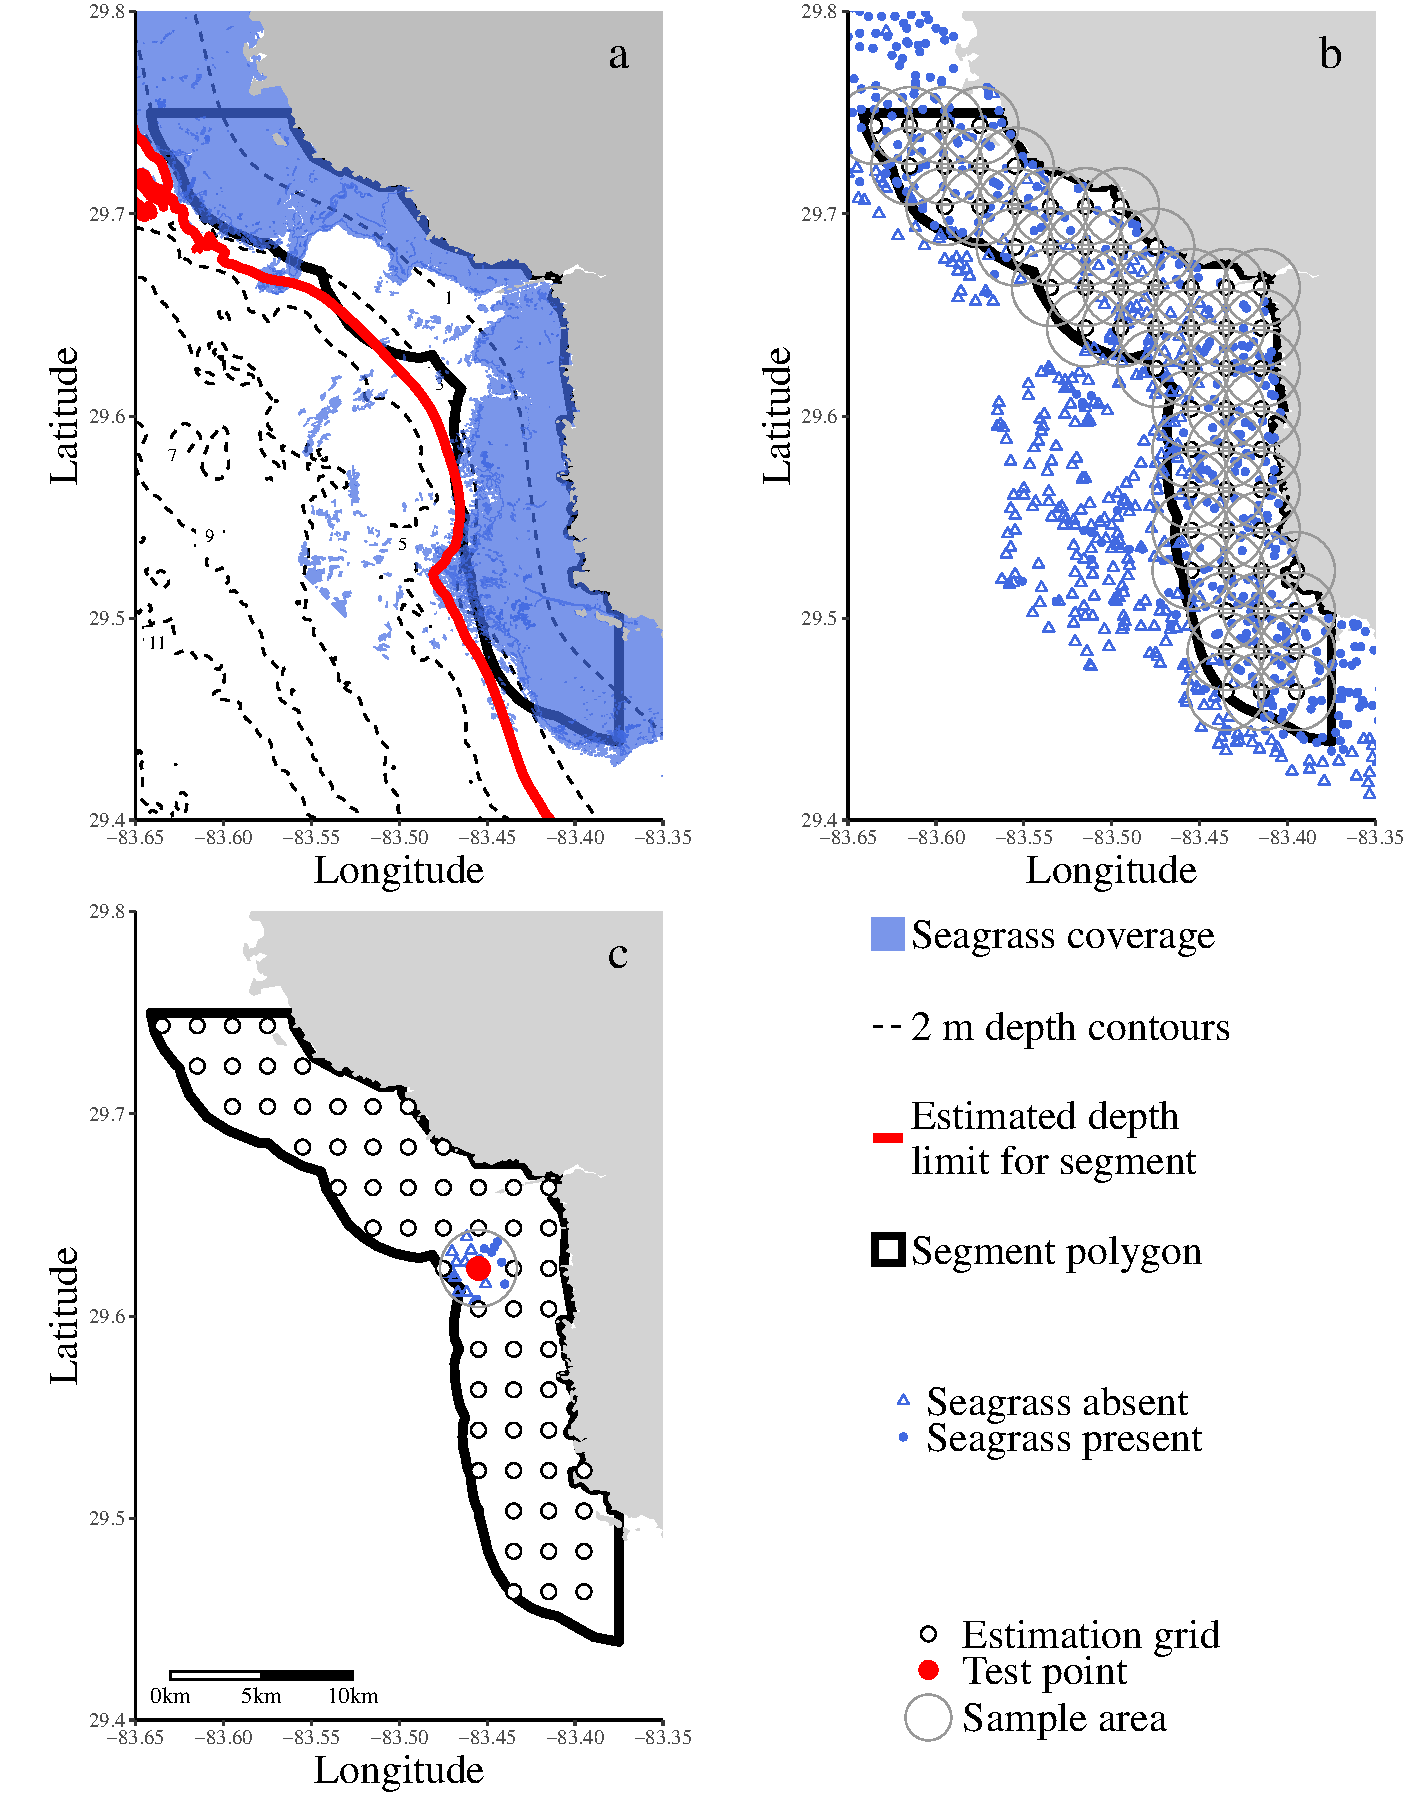
\includegraphics[width=0.9\textwidth]{figs/Fig1.pdf}
\caption{Examples of data and grid locations for estimating seagrass depth of colonization for a region of the Big Bend, Florida.  Subfigure a shows the seagrass coverage and depth contours at 2 meter intervals, including the whole segment estimate for depth of colonization. Subfigure b shows a grid of sampling locations with sampling radii for estimating \ac{doc} and seagrass depth points derived from bathymetry and seagrass coverage layers.  Subfigure c shows an example of sampled seagrass depth points for a test location.  Estimates in \cref{fig:est_ex} were obtained from the test location in subfigure c.}
\label{fig:buff_ex}
\end{figure}

% example of depth of col ests for wbid - big bend 820
\begin{figure}
\centerline{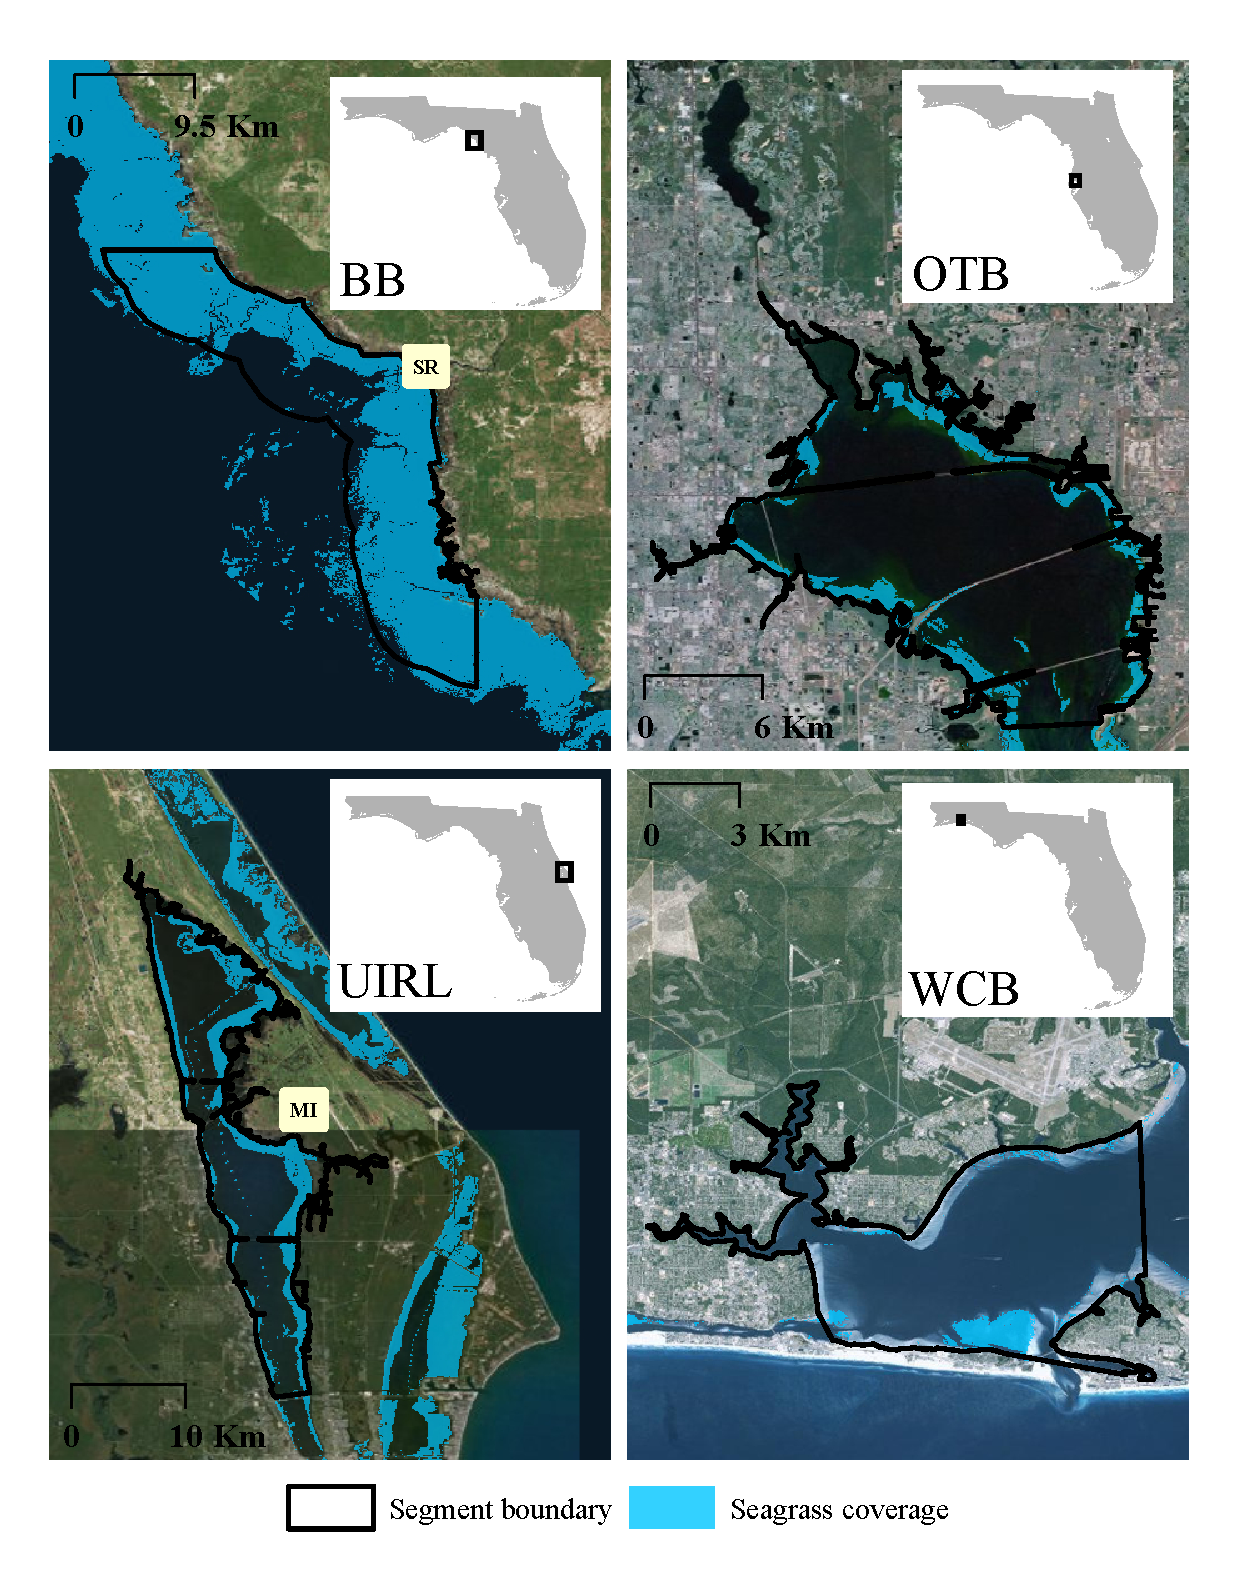
\includegraphics[width = \textwidth]{figs/Fig2.pdf}}
\caption{Locations and seagrass coverage of estuary segments used to evaluate \acl{doc} estimates.  Seagrass coverage layers are from 2006 (BB: Big Bend), 2010 (OTB: Old Tampa Bay), 2009 (UIRL: Upper Indian R. Lagoon), and 2007 (WCB: Western Choctawhatchee Bay). SR: Steinhatchee River outflow, MI: Merritt Island National Wildlife Refuge.}
\label{fig:seg_all}
\end{figure}

% example of estimating seagrass depth of colonization

% example of depth of col ests for wbid - big bend 820
\begin{figure}
\centering
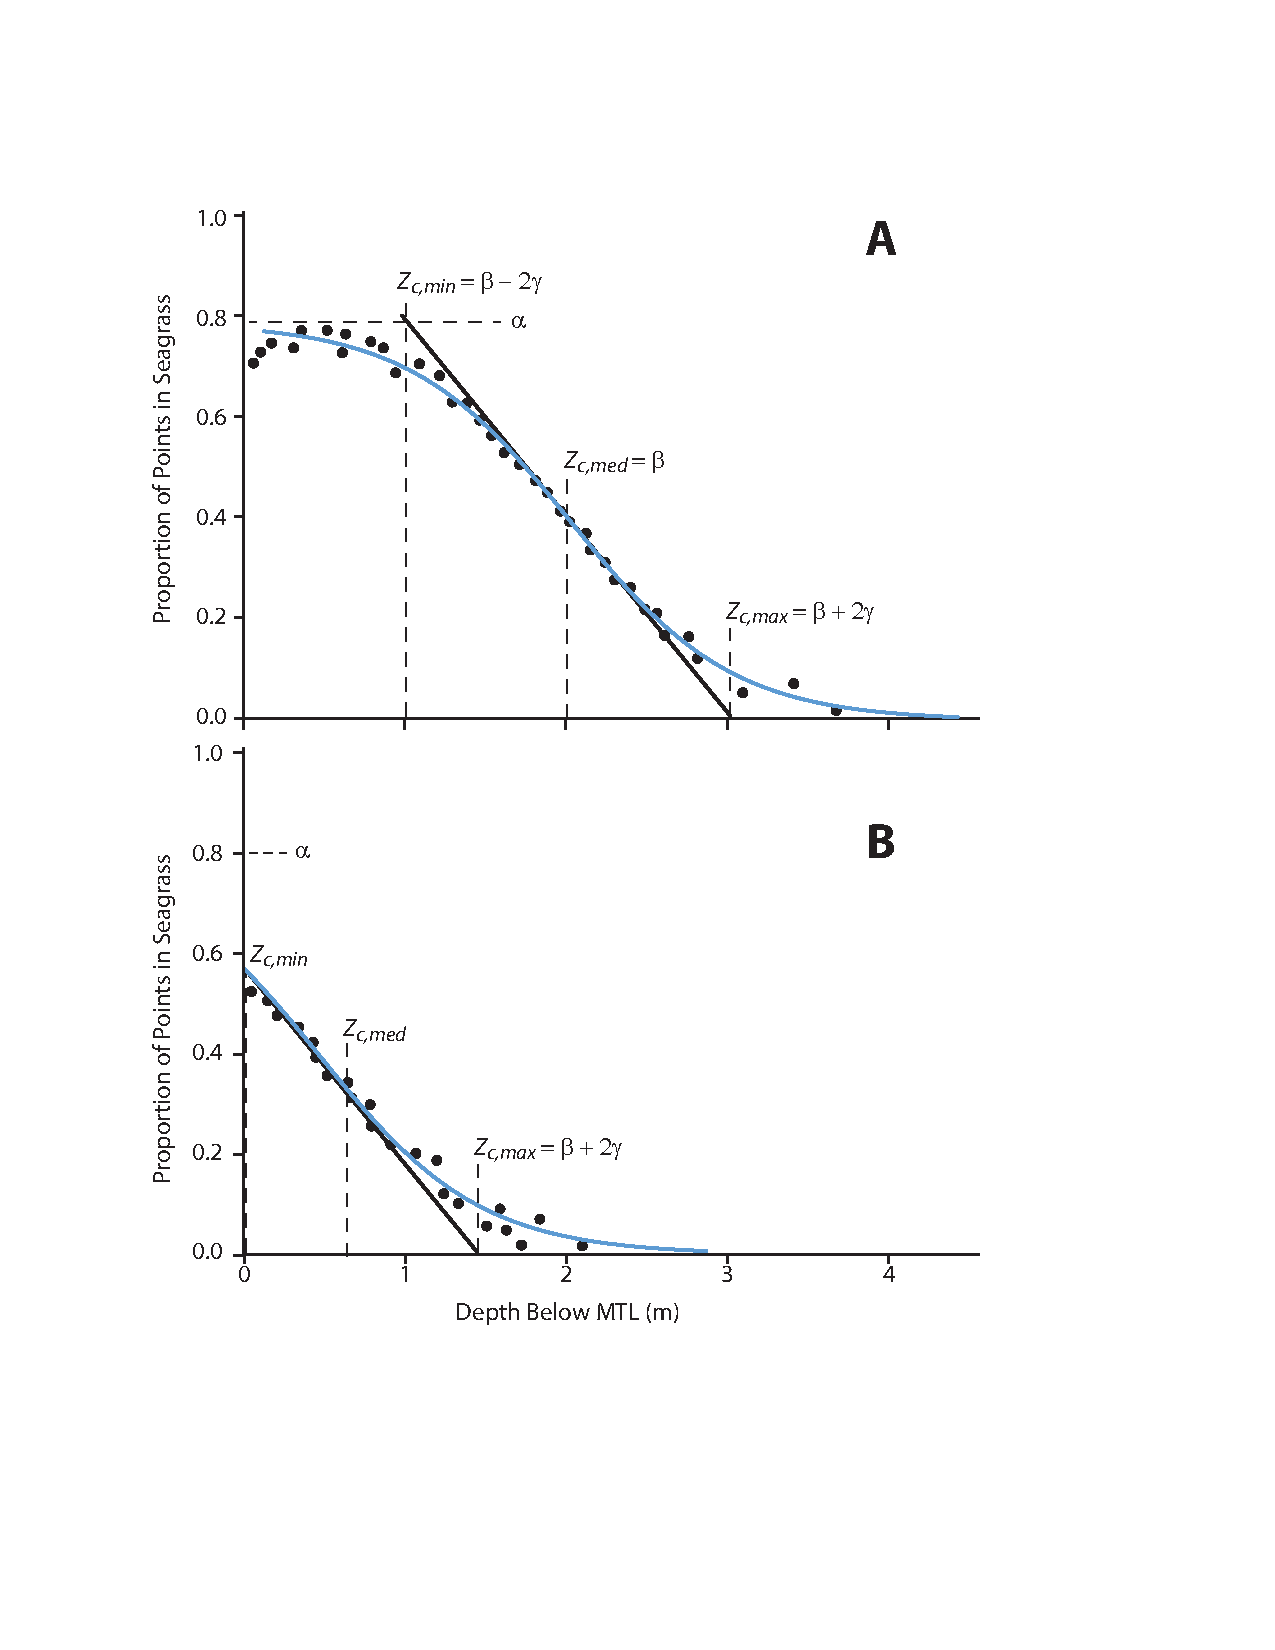
\includegraphics[width=0.85\textwidth]{figs/Fig3.pdf}
\caption{Methods for estimating seagrass depth of colonization using sampled seagrass depth points around a single location. Three depth estimates ($Z_{c,\,min}$, $Z_{c,\,med}$, $Z_{c,\,max}$) are based on a linear curve through the inflection point of a logistic growth curve .  The logistic curve is defined by the parameters $\alpha$, $\beta$, and $\gamma$ and describes the decrease in the proportion of sample points with seagrass as a function of depth below mean tide leavel (MTL).  The top figure shows the estimation method when the linear curve intercepts $\alpha$ at depth greater than zero and the bottom figure shows the estimation method when the linear curve intercepts $\alpha$ at depth less than zero.}
\label{fig:est_ex}
\end{figure}

% grid examples for each segment

\begin{figure}
\centering
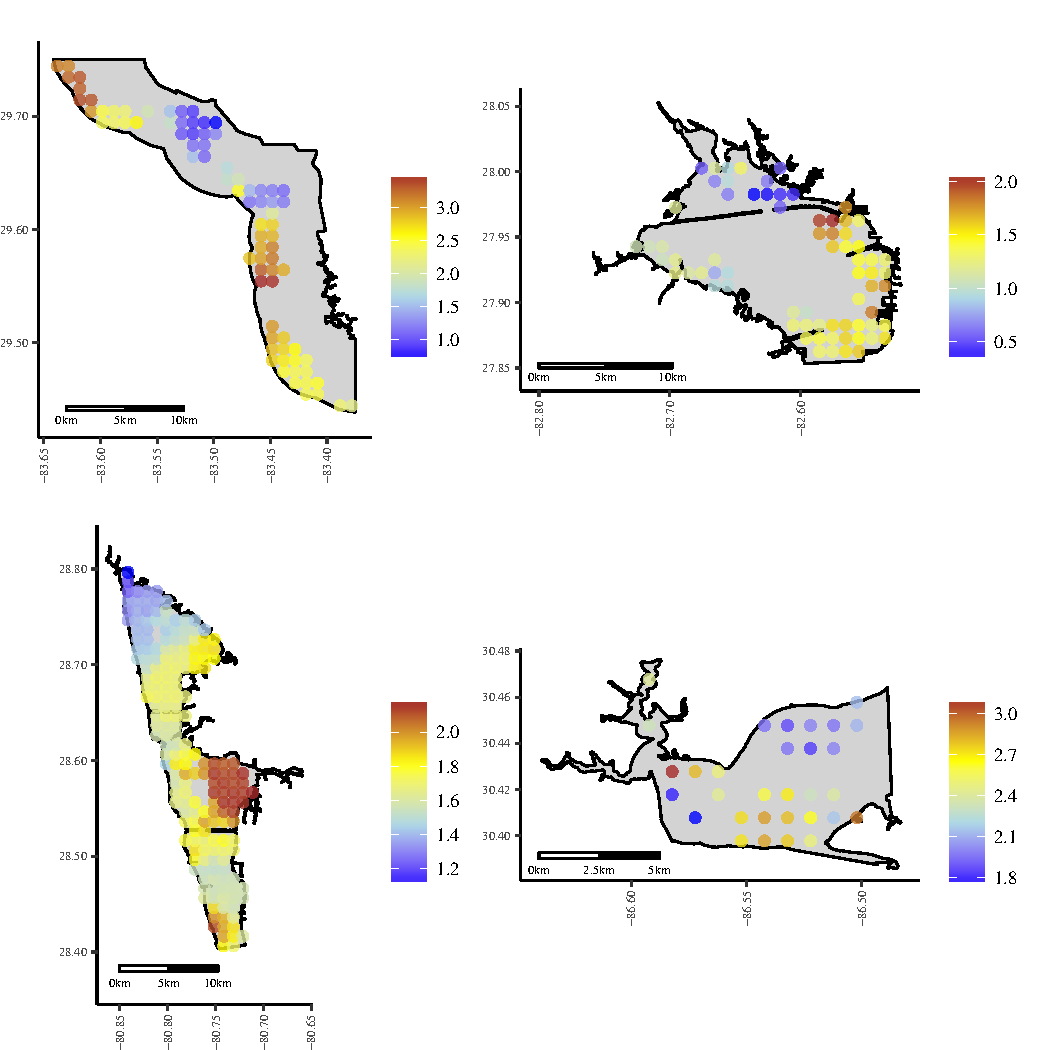
\includegraphics[width = 0.95\textwidth]{figs/Fig4.pdf}
\caption{Spatially-resolved estimates of maximum seagrass depth of colonization (m) for four coastal segments of Florida.  Estimates are assigned to grid locations for each segment, where grid spacing was fixed at 0.02 decimal degrees.  Radii for sampling seagrass bathymetric data around each grid location were fixed at 0.06 decimal degrees. From left to right, top to bottom: Big Bend, Old Tampa Bay, Upper Indian R. Lagoon, Western Choctawhatchee Bay.}
\label{fig:all_ests}
\end{figure}

% satellite estimates of water clarity for choc bay

\begin{figure}
\centering
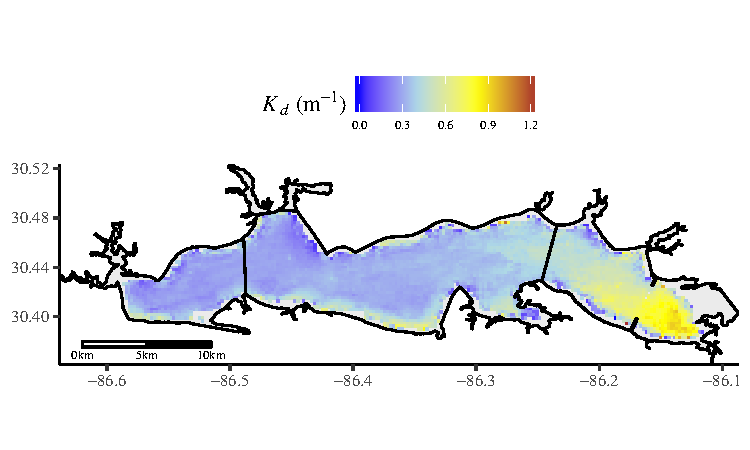
\includegraphics[width = \textwidth]{figs/Fig5.pdf}
\caption{Satellite estimated light attenuation for Choctawhatchee Bay as an average of all years from 2003 to 2007.  See \cref{fig:light_choc} for segment identification.}
\label{fig:kd_choc}
\end{figure}

% satellite estimates of water clarity for Tampa Bay

\begin{figure}
\centering
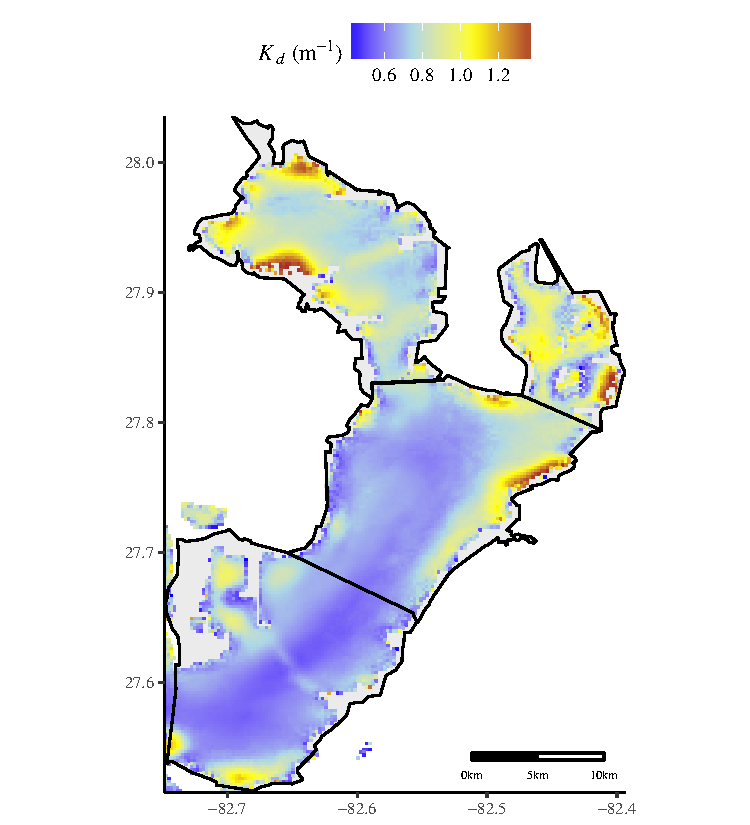
\includegraphics[width = \textwidth]{figs/Fig6.pdf}
\caption{Satellite estimated water clarity for Tampa Bay as an average of all years from 2006 to 2010. See \cref{fig:light_tb} for segment identification.}
\label{fig:clarity_tb}
\end{figure}

% estimated light requirements for Choctawhatchee Bay, z_cmed

\begin{figure}
\centering
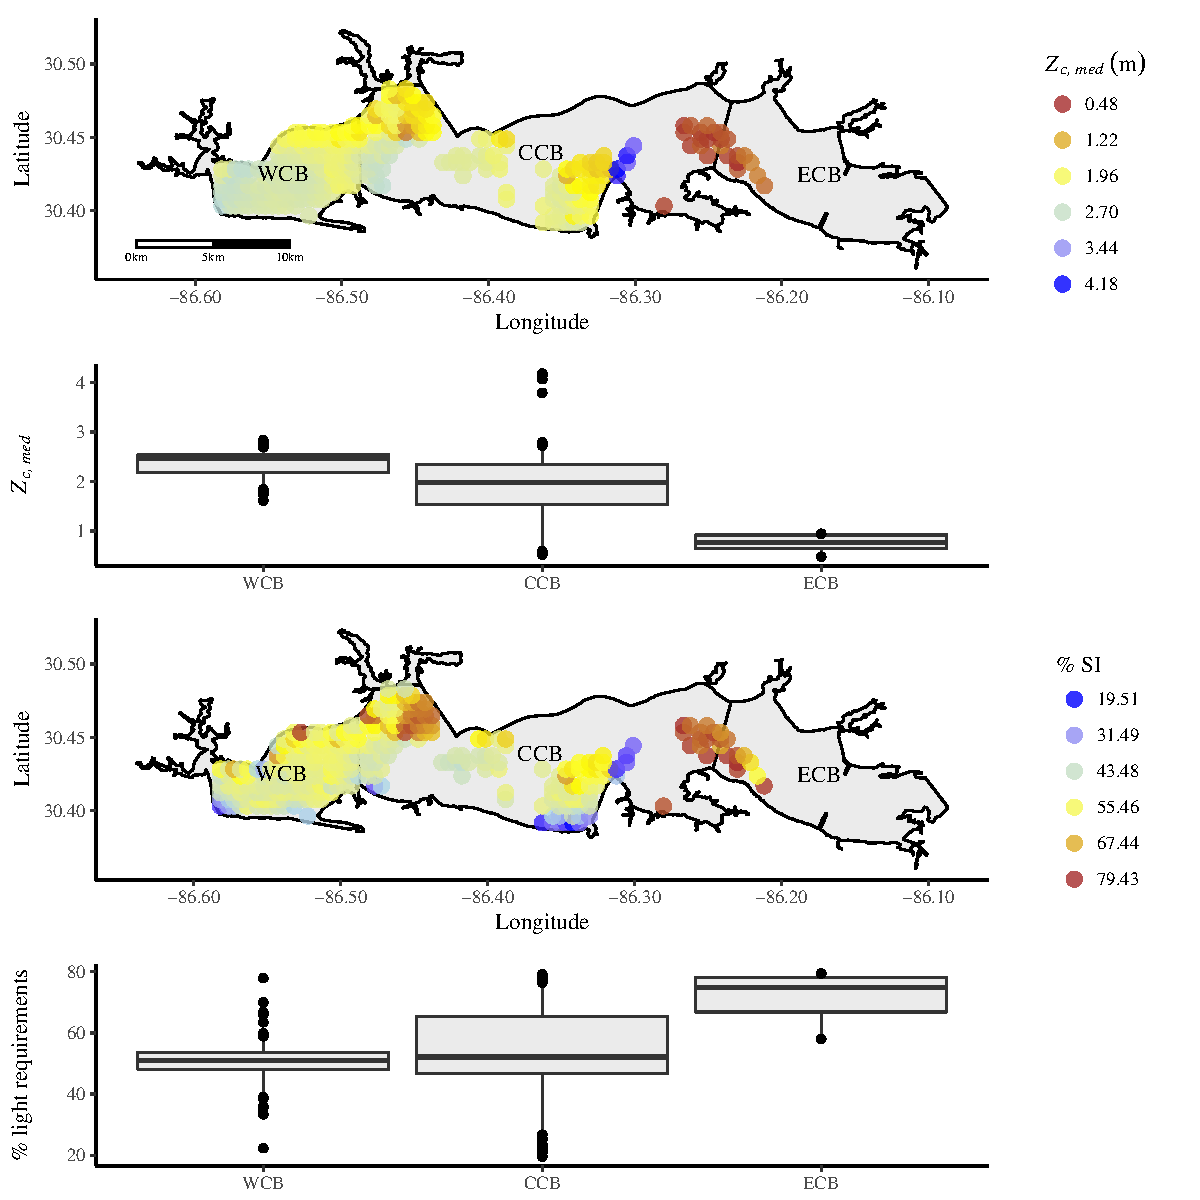
\includegraphics[width = 0.95\textwidth]{figs/Fig7.pdf}
\caption{Estimated median depths of seagrass colonization and light requirements for multiple locations in Choctawhatchee Bay, Florida. Locations are those where water clarity estimates were available from satellite observations and seagrass depth of colonization was estimable using a radius of 0.04 decimal degrees.  Estimates are also summarized by bay segment as boxplots where the dimensions are the 25\textsuperscript{th} percentile, median, and 75\textsuperscript{th} percentile.  Whiskers extend beyond the boxes as 1.5 multiplied by the interquartile range. CCB: Central Choctawhatchee Bay, ECB: East Choctawhatchee Bay, WCB: West Choctawhatchee Bay.}
\label{fig:light_choc}
\end{figure}

% estimated light requirements for Tampa Bay, z_cmed

\begin{figure}
\centering
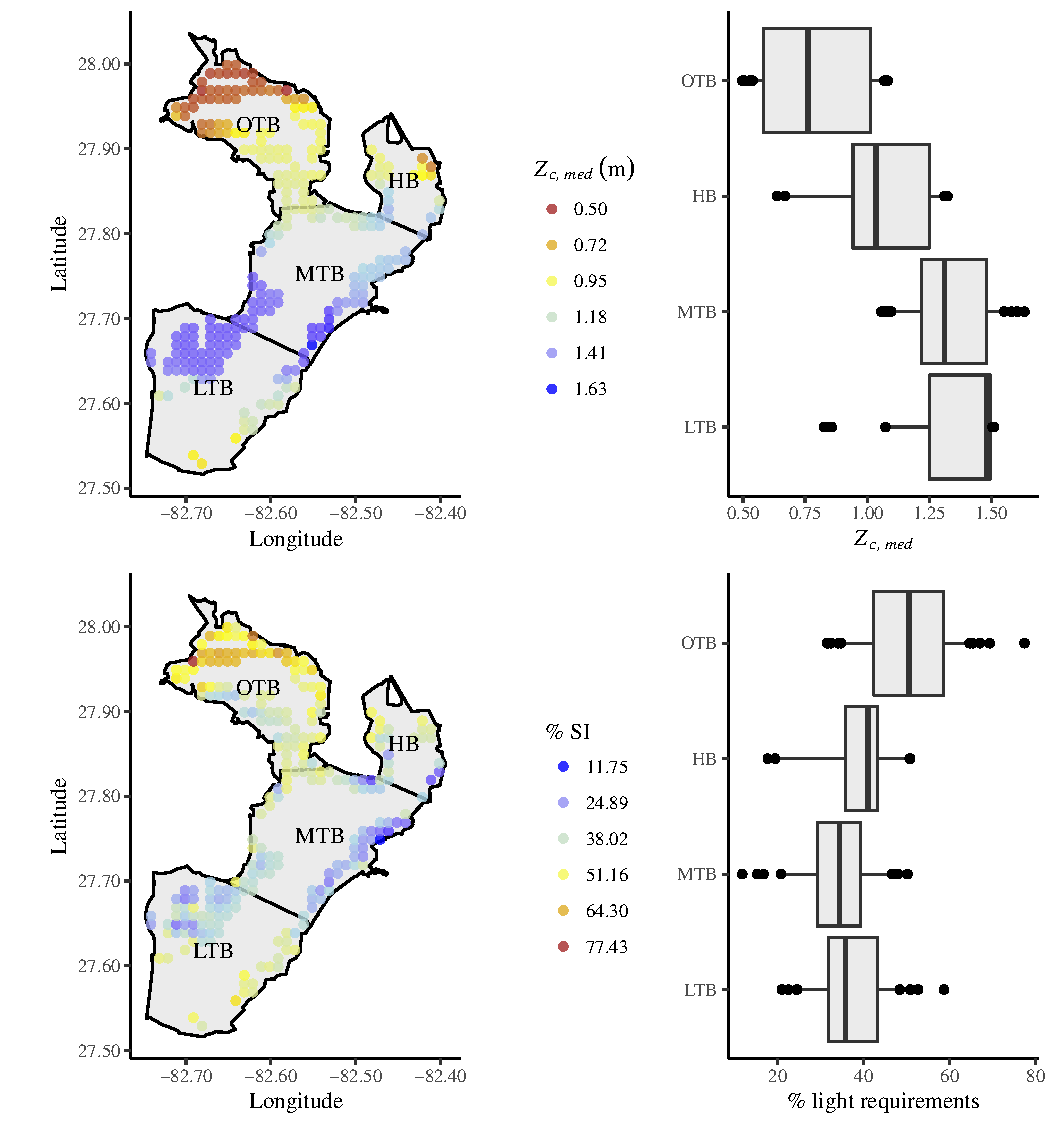
\includegraphics[width = 0.95\textwidth]{figs/Fig8.pdf}
\caption{Estimated median depths of seagrass colonization and light requirements for multiple locations in Tampa Bay, Florida. Locations are those where water clarity estimates were available from satellite observations and seagrass depth of colonization was estimable using a radius of 0.1 decimal degrees.  Estimates are also summarized by bay segment as boxplots as in \cref{fig:light_choc}. HB: Hillsborough Bay, LTB: Lower Tampa Bay, MTB: Middle Tampa Bay, OTB: Old Tampa Bay.}
\label{fig:light_tb}
\end{figure}

% estimated light requirements for Indian River Lagoon, zcmed

\begin{figure}
\centering
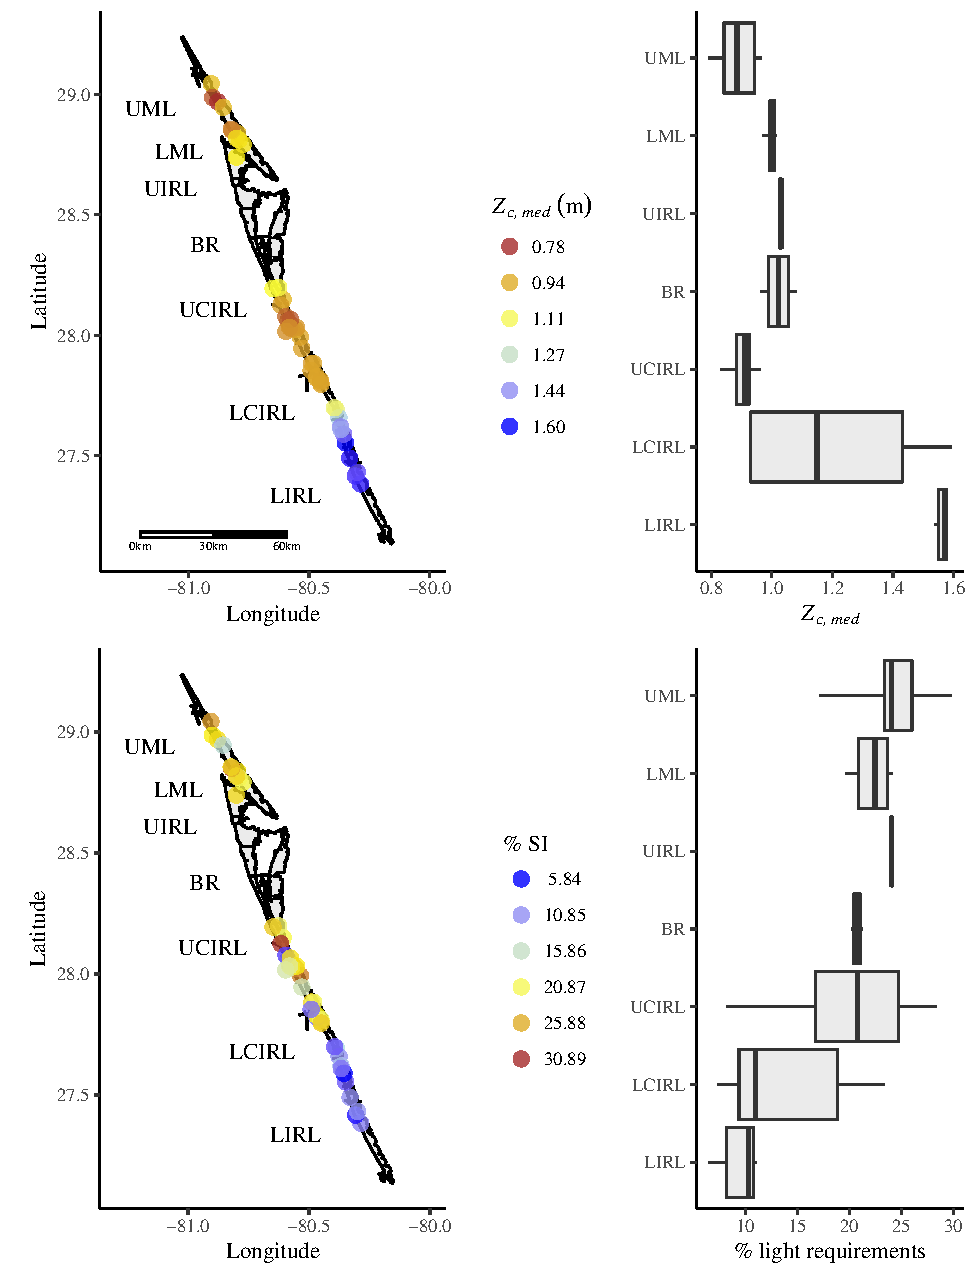
\includegraphics[width = 0.8\textwidth]{figs/Fig9.pdf}
\caption{Estimated median depths of seagrass colonization and light requirements for multiple locations in Indian River Lagoon, Florida.  Map locations are georeferenced observations of water clarity in the Florida \acl{IWR} database, update 40.  Estimates are also summarized by bay segment as boxplots as in \cref{fig:light_choc}. Light requirements are based on averaged secchi values within ten years of the seagrass coverage data and estimated maximum depth of colonization using a radius of 0.15 decimal degrees for each secchi location to sample seagrass depth points. BR: Banana R., LCIRL: Lower Central Indian R. Lagoon, LIRL: Lower Indian R. Lagoon, LML: Lower Mosquito Lagoon, LSL: Lower St. Lucie, UCIRL: Upper Central Indian R. Lagoon, UIRL: Upper Indian R. Lagoon, UML: Upper Mosquito Lagoon.}
\label{fig:light_irl}
\end{figure}
\clearpage

% supplementary material
\beginsupplement

% estimated light requirements for Choctawhatchee Bay, z_cmax

\begin{figure}
\centering
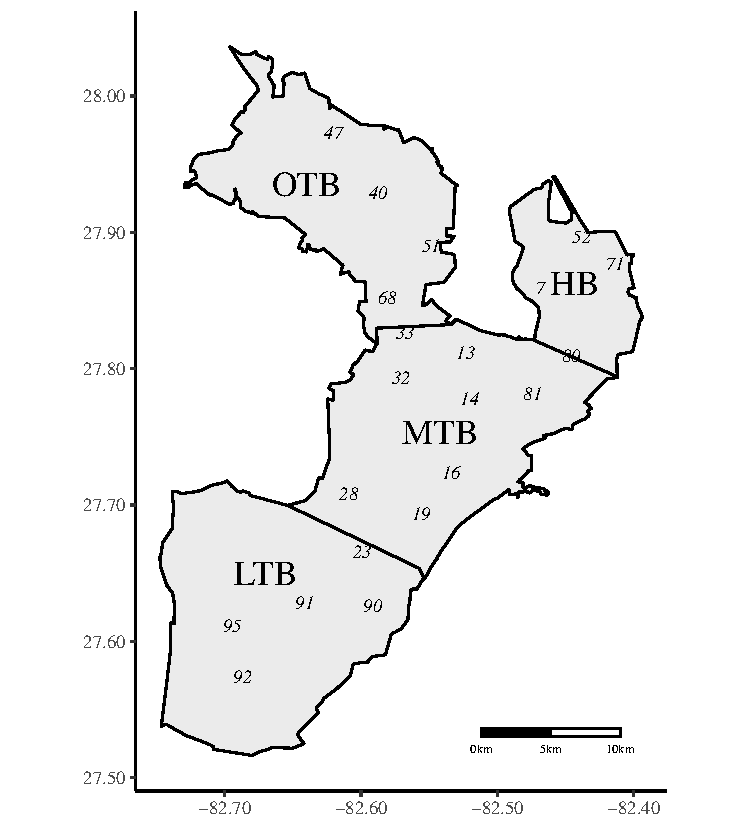
\includegraphics[width = 0.95\textwidth]{figs/FigS1.pdf}
\caption{Estimated maximum depths of seagrass colonization and light requirements for multiple locations in Choctawhatchee Bay, Florida. Locations are those where water clarity estimates were available from satellite observations and seagrass depth of colonization was estimable using a radius of 0.04 decimal degrees.  Estimates are also summarized by bay segment as boxplots where the dimensions are the 25\textsuperscript{th} percentile, median, and 75\textsuperscript{th} percentile.  Whiskers extend beyond the boxes as 1.5 multiplied by the interquartile range. CCB: Central Choctawhatchee Bay, ECB: East Choctawhatchee Bay, WCB: West Choctawhatchee Bay.}
\label{fig:light_choc_zcmax}
\end{figure}

% estimated light requirements for Tampa Bay, z_cmax

\begin{figure}
\centering
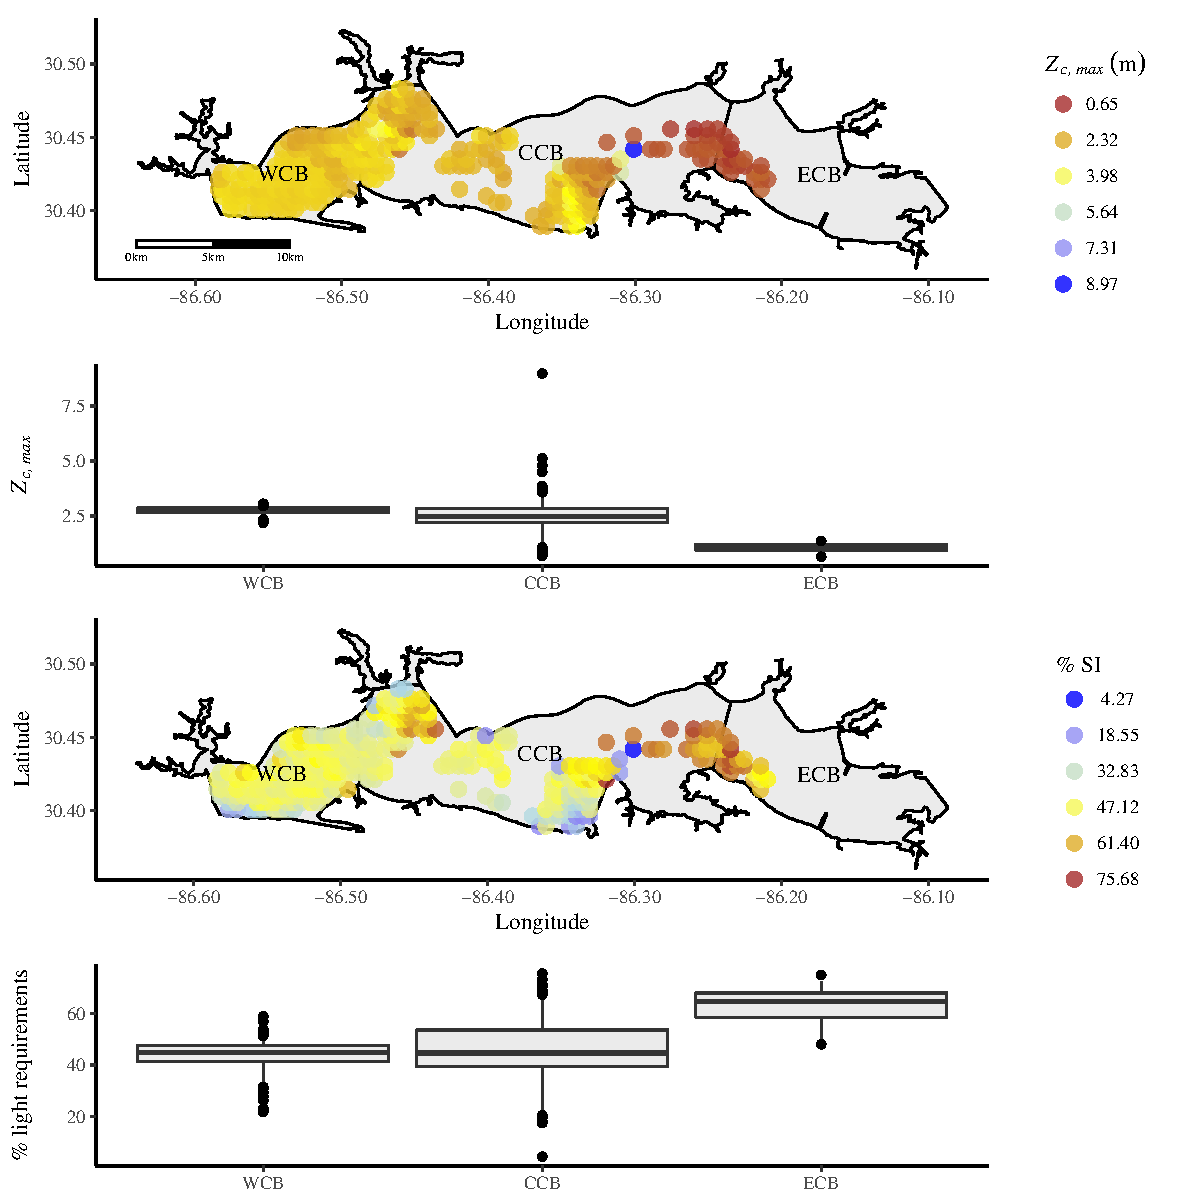
\includegraphics[width = 0.95\textwidth]{figs/FigS2.pdf}
\caption{Estimated maximum depths of seagrass colonization and light requirements for multiple locations in Tampa Bay, Florida. Locations are those where water clarity estimates were available from satellite observations and seagrass depth of colonization was estimable using a radius of 0.1 decimal degrees.  Estimates are also summarized by bay segment as boxplots as in \cref{fig:light_choc}. HB: Hillsborough Bay, LTB: Lower Tampa Bay, MTB: Middle Tampa Bay, OTB: Old Tampa Bay.}
\label{fig:light_tb_zcmax}
\end{figure}

% estimated light requirements for Indian River Lagoon, z_cmax

\begin{figure}
\centering
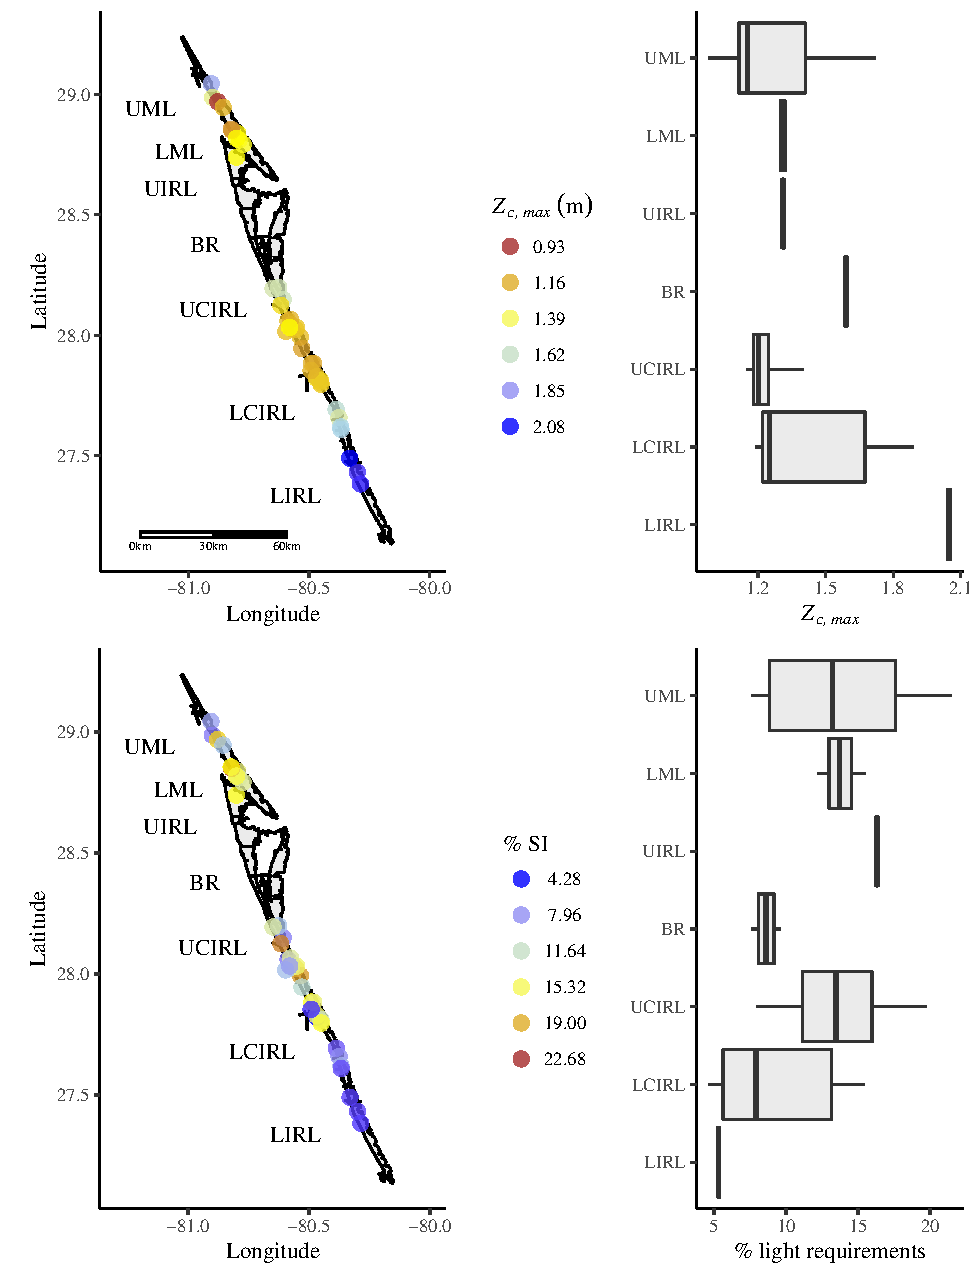
\includegraphics[width = 0.8\textwidth]{figs/FigS3.pdf}
\caption{Estimated maximum depths of seagrass colonization and light requirements for multiple locations in Indian River Lagoon, Florida.  Map locations are georeferenced observations of water clarity in the Florida \acl{IWR} database, update 40.  Estimates are also summarized by bay segment as boxplots as in \cref{fig:light_choc}. Light requirements are based on averaged secchi values within ten years of the seagrass coverage data and estimated maximum depth of colonization using a radius of 0.15 decimal degrees for each secchi location to sample seagrass depth points. BR: Banana R., LCIRL: Lower Central Indian R. Lagoon, LIRL: Lower Indian R. Lagoon, LML: Lower Mosquito Lagoon, LSL: Lower St. Lucie, UCIRL: Upper Central Indian R. Lagoon, UIRL: Upper Indian R. Lagoon, UML: Upper Mosquito Lagoon.}
\label{fig:light_irl_zcmax}
\end{figure}

\end{document}
